Para llevar a cabo esta caracterización de los SiPM se ha necesitado de cierta instrumentación la cual se especifica a continuación:

\begin{enumerate}
\item {} En primer lugar se necesitaba una \textbf{cámara de control de temperatura}. 
\newline
Dado que la cámara existente en el laboratorio del IFIC no estaba configurada tuvo que utilizarse la camara que se encontraba en el IFIMED. Esta cámara (marca DYCOMETAL, modelo CCM 81) se ve reflejada en la figura nueve izquierda.

Este sistema dispone de un panel de control con el que poder especificar la temperatura y humedad a la que queremos trabajar en el interior de la cámara. Sin embargo, para asegurar el correcto funcionamiento de la cámara debiamos trabajar siempre en la zona 1 de acuerdo al diagrama de fases existente en la ficha técnica de la cámara, mostrado en la figura nueve derecha. Posee un interior metálico que nos permite una rápida estabilidad ante posibles cambios de las condiciones en su interior y, además, actua a modo de jaula de Faraday. 

\begin{figure}[htb]
\centering
{
%\subfloat[Espectro de emisión]
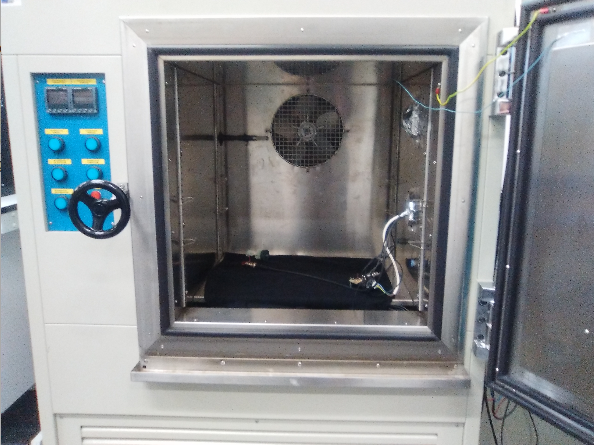
\includegraphics[scale=0.3]{InteriorTemperatura.png} 
}
{
%\subfloat[Espectro de emisión]
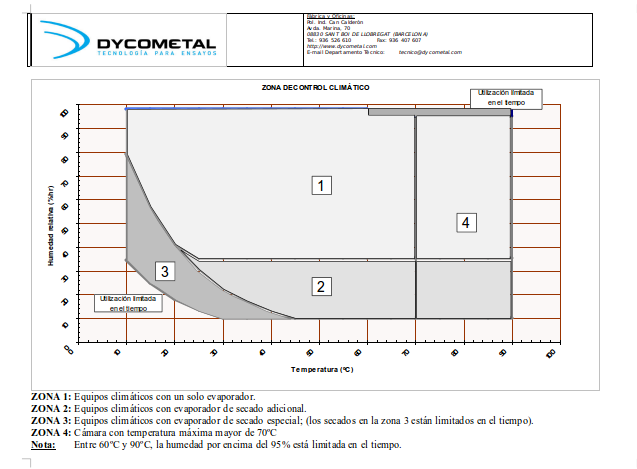
\includegraphics[scale=0.3]{FichaTecnica.png} 
}
\caption{\textbf{Figura 9}.-Sistema de control de temperatura y diagrama de fases}
\end{figure}

Su incertidumbre se encontraba en 0.1 grados para la temperatura y 0.5\% para la humedad relativa. Estas incertidumbres se determinaron observando la oscilación  máxima en la pantalla del panel de ambos parámetros tras llegar a la estabilidad en el interior de la cámara.

En el interior de esta cámara se encontraba nuestra fuente que proporcionaba la señal de entrada del sistema que pretendíamos medir con el SiPM, el propio SiPM, la tarjeta de conversión intensidad-voltaje y cableado que hacía posible la interacción con estos dispositivos. Además hay que tener en cuenta que esta cámara no actuaba como caja negra, por lo que para conseguir reducir la posible entrada de luz del exterior se taparon todas las posibles fisuras del sistema con cinta metálica y, ademas, se cubrió el experimento con una tela negra especial. Con todo esto conseguiamos reducir el background del sistema hasta un nivel adecuado.

\item {} En segundo lugar se necesitabamos instrumentos nos permitiesen alimentar tanto el SiPM como la tarjeta de conversión intensidad-voltaje. Se utilizo  un \textbf{electrometro} (marca KEITHLEY, modelo 6517B) para alimentar el SiPM y un \textbf{generador de tensión} (marca ISO-TECH, modelo IPS-4303) para alimental la tarjeta de conversión.

Se utilizo el electrómetro para el SiPM ya que este dispone de rango de voltajes mayor, necesario para alimentar al SiPM. Por el contrario, el ISO-TECH solo dispone de una tensión máxima de 30V insuficiente para alimentar al SiPM pero suficiente para alimentar la tarjeta. Poseen una resolución inferior inferior al milivoltio e inferior a 0.1 voltios respectivamente, suficiente para considerarlos constantes ya que las ganancias que dependen de estos (ganancia del SiPM y de la tarjeta respectivamente) necesita variaciones superiores para modificarse de forma apreciable.

\item {} En tercer lugar se necesitaba una \textbf{fuente} que simulase la emisión de los fotones de la fibra centelleadora. 
\newline
Se utilizo un \textbf{diodo LED} (de la empresa Roithner Laser technik) que emitía fotones con una longitud de onda de 435 nm, correspondiente al azul. Este es la longitud de onda que necesitabamos en nuestro experimento para calibrar el SiPM ya que corresponde a la longitud de onda a la cual el espectro de emisión de las fibras centelleadoras BCF-12 tiene su máximo.

%\newpage
\item {} En cuarto lugar, para alimentar este diodo LED, se necesito un \textbf{generador de pulsos} (marca Agilent, modelo 33250A). Este generador de señales nos permite especificar la forma del pulso que pretendemos proporcionar y sus características. Este tenía que ser capaz de formar un pulso suficientemente estrecho para que el SiPM detectase unos pocos fotones. 

En concreto alimentaremos el diodo LED con un pulso cuadrado. Los parámetros que nos permite especificar el generador de señales para un pulso de esta forma son frecuencia (o periodo), high level (o amplitud), low level, offset, anchura del pulso y tiempo de decaimiento. Para nuestro estudio los valores de estos parámetros que nos daban un mejor resultado desde el punto de vista experimental fueron una frecuencia de 20 Hz, high level de 2.275 V, low level de 1 V, offset de 1.638 $V_{dc}$, anchura del pulso de 12 ns y tiempo de decaimiento de 5 ns.

Este generador de señal nos proporciona una segunda señal denominada señal de sincronización la cual podemos utilizar como trigger para determinar el instante de tiempo en el que se activa la señal.

\item {} En quinto lugar utilizamos un \textbf{SiPM} para detectar los fotones emitidos por el LED. En concreto se utilizo el modelo S13360-1375CS de hamamatsu, que es un fotomultiplicador cerámico de silicio que presenta una ganancia teórica de $G=4 \cdotp 10^6$ y una eficiencia de fotodetección teórica del 50\% a 25 grados y $V_{ov}=V_{op}-V_{bd}=3V$. Este tiene un rango espectral de [270-900] nm.

Esta compuesto por un total de 285 pixels de 75 $\mu m$ cada uno dando lugar a una superficie total activa de 1.3x1.3 $mm^2$ frente a su superficie total que es de 6x5 $mm^2$. Puede verse reflejado en la figura diez izquierda. 

\item {} Hay que tener en cuenta que el SiPM nos proporciona un pulso de intensidad a la salida y  necesitamos convertir este en un pulso de voltaje para, de esta forma, poder introducirla al osciloscopio para realizar el posterior análisis. Para ello emplearemos en sexto lugar una \textbf{tarjeta conversora} de intensidad en voltaje que puede verse reflejada en la figura diez derecha. 

\begin{figure}[htb]
\centering
{
%\subfloat[Espectro de emisión]
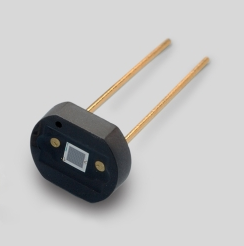
\includegraphics[scale=0.4]{SiPM.png} 
}
{
%\subfloat[Espectro de emisión]
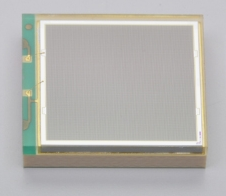
\includegraphics[scale=0.5]{SiPMfinal.png} 
}
{
%\subfloat[Espectro de emisión]
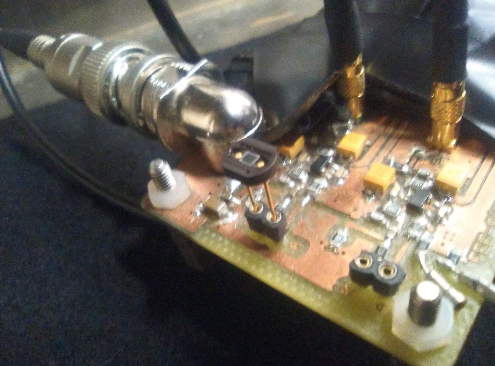
\includegraphics[scale=0.4]{tarjeta.png} 
}
\caption{\textbf{Figura 10}.-SiPMs y tarjeta de conversora intensidad-voltaje}
\end{figure}

\item {} Finalmente vimos que, únicamente alimentando la tarjeta, antes de alimentar el SiPM y la led, obteníamos una perturbación externa a nuestro experimento. Esta se presenta en la figura once. 

\begin{figure}[hbtp]
\centering
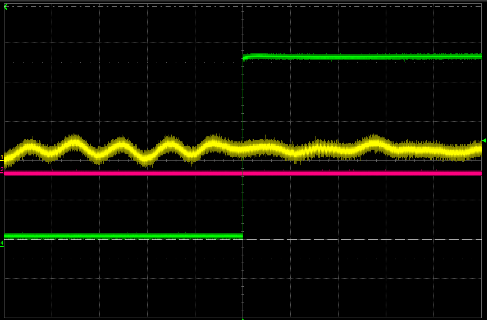
\includegraphics[scale=0.4]{ruido.png}
\caption{\textbf{Figura 11}.- Ruido electrónico}
\end{figure}

Se intento caracterizar esta señal de perturbación ajena a nuestro experimento y, a priori, de origen desconocido. Tenía una amplitud máxima de 4 mV y una frecuencia bastante irregular entorno al MHz. Finalmente se vio que era debido por una parte a la emisión producida por la antenas de radiotelevisión valenciana y, por otra parte, de las distintos intrumentos electrónicos conectados a la red eléctrica del IFIC, ya que esta posee una toma a tierra bastante irregular. 

Con la presencia de este ruido no podíamos realizar medidas ya que introducía una componente de ruido tal que estropeaba por completo el resultado de la medida. Con el fin de solucionar este problema se dispuso de un \textbf{filtro pasa banda} (marca..., modelo...) para eliminar este ruido.

\item {} Finalmente, como se ha mencionado anteriormente, necesitamos una \textbf{manta negra} especial que apantallase la entrada de fotones del exterior, ya que el sistema de control de temperatura no actuaba como caja negra.

Una alternativa podría haber sido introducir una caja negra en el interior del sistema de control de temperatura y introducir el diodo Led, el SiPM y la tarjeta en su interior. Sin embargo de esta forma no conseguimos un control de la temperatura y humedad en su interior.

\end{enumerate}
